\documentclass{article}

\usepackage{graphicx}
\usepackage{amsmath}
\usepackage{amssymb}
\begin{document}
\textbf{Siddharth Bhat (20161105)}

\section{Q7}
\subsubsection{Q7.1}
$SL_x(E)$ for a shared lock by transaction $x$ on elem $E$. $U_x(E)$ for
unlock by transaction $x$ on elem $E$.

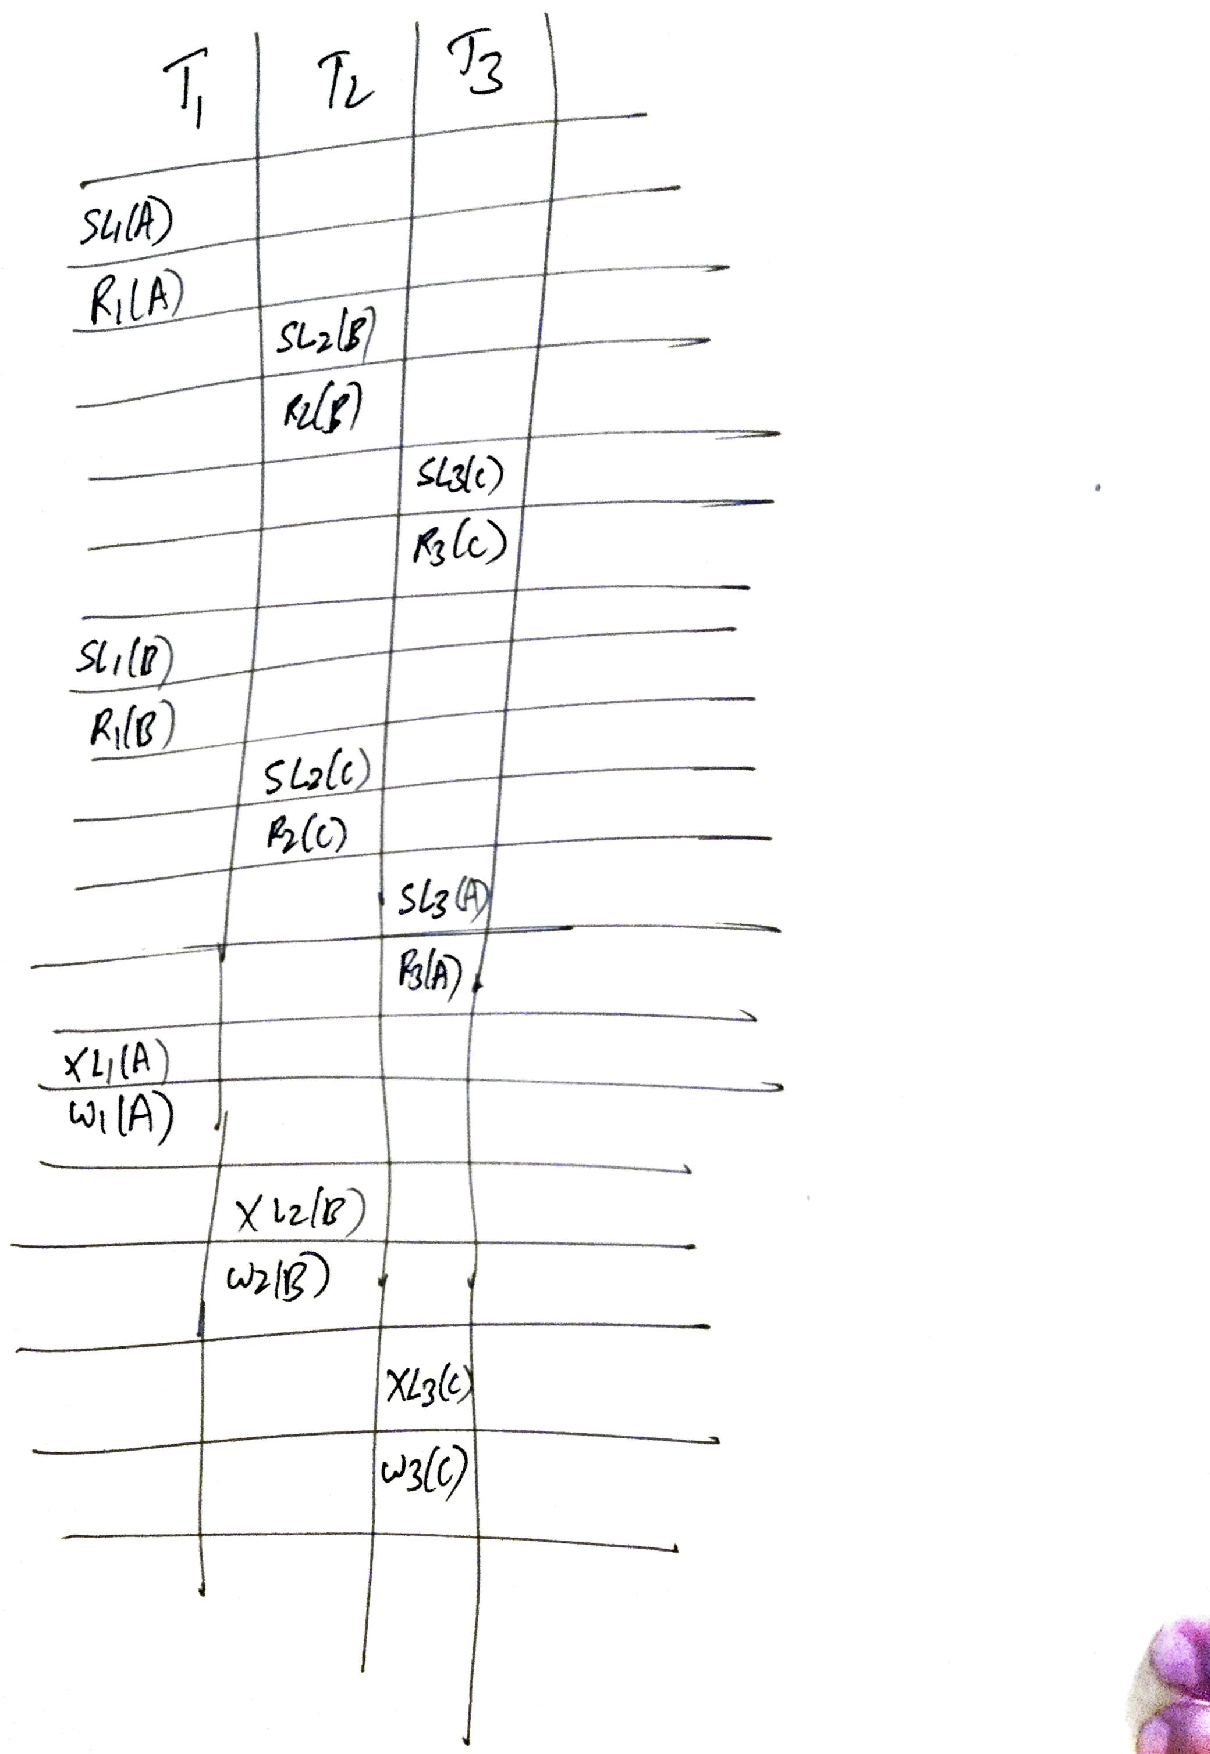
\includegraphics[width=0.8\textwidth]{db-q71.pdf}

All locks are accepted, since there are no conflicting locks.

\subsubsection{Q7.2}

Table will be the same as for the above, since we did not have any read action
which was followed by a write action of the same element by the same
transaction.


\subsubsection{Q7.3}


\section{Q8}
\begin{align*}
    &r_1(O_1) \mapsto \text{$T_1$ puts }IS(B_1); S(O_1); \texttt{release} \\
    &r_2(O_2) \mapsto \text{$T_2$ puts }IS(B_1); S(O_2); \texttt{release}\\
    &r_3(O_1) \mapsto \text{$T_3$ puts }IS(B_2); S(O_3); \texttt{release}\\
    &w_1(O_3) \mapsto \text{$T_1$ puts }IX(B_2); X(O_3); \texttt{release}\\
    &w_2(O_4) \mapsto \text{$T_2$ puts }IX(B_2); X(O_4); \texttt{release}\\
    &w_3(O_5) \mapsto \text{$T_3$ puts }IX(B_2); X(O_5); \texttt{release}\\
    &w_1(O_2) \mapsto \text{$T_1$ puts }IX(B_2); X(O_3); \texttt{release}\\
\end{align*}
\section{Q9}
\subsubsection{9.1}
In Undo Logging Logging, we need to write all we need to write all modified
data to disk before committing a transaction.  This may need a large number of disk
I/O’s. This is unlike the case of Redo logging, which allows changes to be
present in-memory; only need to flush changes before committing.

\subsubsection{9.2}
Selinger optimization improves upon DP approach by keeping for
each  not only the plan of least cost, but also plans that have higher
cost but produce a result that is sorted in an order that may
be useful for parent queries.
\subsubsection{9.3}

View serializable: If a given schedule is found to be view equivalent to some serial schedule. Alternatively,
  there are no cycles in the dependency graph.
Conflict serializable: If there are no cycles in the conflict graph.


\subsubsection{9.4}

We can use strict 2-phase locking for recoverability. This requires that
in addition to the lock being 2-Phase, all Exclusive(X) Locks held by the
transaction be released until after the Transaction Commits.

\subsubsection{9.5}
Database operations are in fact relational algebra operations. These
operations are pure mathematical expressions, and are generally reads or
writes into disjoint pieces of data. This makes them naturally parallelizable.


\subsubsection{9.6}
File system does not generally have multiple readers and writers to a single
file. It also does not need to manage structured data. Hence, many of the ACID
like concerns simply do not occur in the case of a file system.

\subsubsection{9.7}
the commit bit for X is true if and only if the most recent
transaction to write X has already committed. The purpose of this bit
is to avoid a situation where one transaction T reads data written by
another transaction U, and U then aborts. This problem, where T makes
a "dirty read" of uncommitted data, certainly can cause the database
state to become inconsistent, and any scheduler needs a mechanism to
prevent dirty reads.

\subsubsection{9.8}
\begin{itemize}
        \item  Two-phase locking - 2PL.
        \item General lock based solutions.
        \item Timestamp ordering.
        \item Validation based concurrency control.
\end{itemize}

Increment based locking is good in this case because it allows to add or subtract a constant
from an element, which is what most kinds of bank transaactions are. Increment locks on the same
element do not conflict with each other.
\subsubsection{9.9}
recovery manager will have to DODO
\subsubsection{9.10}
all trees of n vertices is $n^{n-2}$. Number of left-deep trees is $n!$.
$n^{n-2}$ is much larger than $n!$.


\end{document}
